
\documentclass{ppgeesa}

%%%%%%%%%%%%%%%%%%%%%%%%%%%%%%%%%%%%%%%%%%%%%%%%%%%%%%%%%%%%%%%%%%%%%%%%%%%%%%%%%%%%%%%%%%%%%%%%%%%%%%%%%%%%%%%%%

\usepackage[latin1]{inputenc}
\usepackage{graphicx}
\usepackage{hyperref}
\usepackage{tikz}
\usepackage{amsmath}
\usepackage{listings}

\lstset{stepnumber=2, frame=single,tabsize=2, breaklines=true, basicstyle=\footnotesize}

\hypersetup{
	colorlinks,
	debug=true,
	linkcolor=black,  %%% cor do tableofcontents, \ref, \footnote, etc
	citecolor=red,  %%% cor do \cite
	urlcolor=blue,   %%% cor do \url e \href
	bookmarksopen=true,
	pdftitle={Controle Robusto},
	pdfauthor={Tassiano Neuhaus},
	pdfsubject={Sistemas de controle multivari�veis},
	pdfkeywords={Controle Robusto}
	%pdfpagemode=FullScreen
}

%%%%%%%%%%%%%%%%%%%%%%%%%%%%%%%%%%%%%%%%%%%%%%%%%%%%%%%%%%%%%%%%%%%%%%%%%%%%%%%%%%%%%%%%%%%%%%%%%%%%%%%%%%%%%%%%%


\begin{document}

\title{Controle Robusto e Caracteriza��o de incertezas}

\author{Tassiano Neuhaus\\
{\small Universidade Federal do Rio Grande do Sul - Departamento de Engenharia El�trica\\Av. Osvaldo Aranha, 103 - Bairro Bom Fim CEP: 90035-190 - Porto Alegre - RS - Brasil}\\
}%\thanks{Tassiano Neuhaus, tassianors@gmail.com, tel +55-51-91760154}}

\maketitle
\thispagestyle{empty}\pagestyle{empty}

\begin{abstract}
Neste trabalho ser� apresentado a caracteriza��o de um sistema sujeito a incertezas. A caracteriza��o
ser� baseada nos seguintes tipos: Polit�picas, limitadas em norma, diagonal e elemento por elemento.

Para cada uma das incertezas caracterizadas ser� projetada uma realimenta��o de estados para minimizar
a norma {\it{$H_2$}} em malha fechada. O mesmo ser� feito para minimizar a norma {\it{$H_{\infty}$}}

Ao fim ser� feita uma breve compara��o entre os resultados obtidos no trabalho.
\end{abstract}

\begin{IEEEkeywords}
Controle Robusto, Incertezas polit�picas, limitadas em norma e diagonais.
\end{IEEEkeywords}

%===============================================================================
\section{Introdu��o}

Neste trabalho ser� apresentado um sistema de para controle de posi��o angular,
manipulado por um motor de corrente continua (DC). O objetivo principal, � estimar
os valores das vari�veis existentes no modelo escolhido para representar este sistema.

Inicialmente ser� explicado o processo de escolha do modelo que representa a din�mica
deste sistema (Se��o (\ref{sec:modelling})). Ser� explicitado quais considera��es sobre
o sistema foram feitas para se obter o modelo que ser� utilizado nas se��es seguintes, 
para determinar os par�metros.

Em seguida, ser� utilizado o m�todo dos M�nimos quadrados (MQ), para estimar o sistema, 
considerando-se para isso que o ruido sobre o sistema sofre influ�ncia dos mesmos polos
que est�o na planta, ou seja, que o modelo para o sistema se comporta como um modelo ARX.
Nesta mesma se��o (\ref{sec:mmq}) ser� apresentado os resultados para o mesmo sistema, 
baseado nos mesmos dados, mas para um modelo que n�o representa o sistema f�sico, ou que 
n�o consegue representa-lo.

Na se��o (\ref{sec:iv}) ser� apresentado o m�todo das vari�veis instrumentais, para estimar
os valores do par�metro para o modelo. Da mesma forma que para o m�todo dos MQ, ser�
utilizado um modelo que n�o representa o sistema real, e este m�todo ser� aplicado para 
determinar a qualidade dos resultados obtidos.

Ao fim, ser� apresentado uma breve discuss�o sobre os resultados obtidos em ambos os m�todos
utilizados, e as considera��es finais.


\section{Caracteriza��o}
\label{sec:caracterization}
%===============================================================================

As incertezas presentes em um modelo matem�tico podem ter diversas origens:

\begin{itemize}
\item As varia��es param�tricas lentas e continuas devido ao envelhecimento
de certos elementos f�sicos, ou bruscas devido a mudan�a no ponto de opera��o.

\item Erro de estimativa nos par�metros do modelo

\item Hip�teses simplificarias na modelagem do sistema e/ou din�micas negligenciadas
para redu��o do modelo.
\end{itemize}

As incertezas s�o classificadas da seguinte forma:

\begin{itemize}
\item {\bf{Param�tricas}}: Devido as varia��es ou desconhecimento de certos valores
f�sicos do sistema. Ex: Massa, temperatura ...

\item {\bf{N�o Param�tricas}}: Devido a din�micas desconhecidas ou n�o identificadas
no procedimento de identifica��o do sistema.

\item {\bf{Estruturais}}: Aquelas sobre as quais tem-se uma informa��o precisa sobre 
a maneira que elas agem sobre o sistema.

\item {\bf{N�o Estruturais}}: S�o aquelas onde a �nica informa��o � o limite superior
de sua norma.
\end{itemize}

O sistema sujeito as incertezas referidas anteriormente podem ser representados na forma
de Equa��es de estados como em {\ref{eq:model_sistem}

\begin{equation}
\left \{ \begin{matrix}
\dot{x}(t)=Ax(t)+Bu(t) & A \in \mathbf{A}\\ 
y(t)=Cx(t) & B \in \mathbf{B}
\end{matrix} \right.
\label{eq:model_sistem}
\end{equation}

Onde $ \mathbf{A} e \mathbf{B}$ � o conjunto de par�metros que s�o formados pelas
varia��es das incertezas dos par�metros.

%===============================================================================
\subsection{Polit�pica}
\label{sec:carac_politopica}

Uma incerteza � dita do tipo polit�picas se $ \mathbf{A} e \mathbf{B}$ tem as estruturas
seguintes:

\begin{equation}
\mathbf{A}_p \equiv {A: A \in \mathbf{Co}(A_i); i=1,...,na}
\nonumber
\end{equation}

\begin{equation}
\mathbf{B}_p \equiv {B: B \in \mathbf{Co}(B_j); j=1,...,nb}
\nonumber
\end{equation}

Onde $\mathbf{Ca}$ � um envelope convexo, ou seja, uma combina��o linear convexa.

De forma equivalente temos que um sistema de incertezas do tipo polit�picas podem 
ser representados por (\ref{eq:carac_politopico}.

\begin{equation}
\mathbf{A}_p \equiv {A: A = \sum_{i=1}^{na}\alpha_i(t)A_i;\alpha_i\geq 0;\sum_{i=1}^{na}\alpha_i(t)=1; \forall t\geq  0}
\label{eq:carac_politopico}
\end{equation}

As incertezas polit�picas s�o consideradas {\it{estruturais}} pois pode-se facilmente
estimar as varia��es admitidas para cada elemento das matrizes que definem o conjunto
de modelos.


%===============================================================================
\subsection{Limitada em norma}
\label{sec:carac_limit_norma}

Incertezas limitadas em norma possuem a seguinte estrutura:

\begin{equation}
\mathbf{A}(\Delta(t))\equiv \{A: A=A_0+\Delta A+D \Delta (t)E_A\}
\label{eq:carac_limit_norma_a}
\end{equation}

\begin{equation}
\mathbf{B}(\Delta(t))\equiv \{B: B=B_0+\Delta B+D \Delta (t)E_B\}
\label{eq:carac_limit_norma_b}
\end{equation}

Com $ \left \| \Delta (t) \right \| \leq 1$.

De maneira equivalente o sistema de equa��es de estado fica como em (\ref{eq:carac_lim_norma_sis}).

\begin{equation}
\begin{cases} 
\dot{x}(t)=A_0x(t)+B_0u(t)+Dp(t)\\
q(t)=E_Ax(t)+E_Bu(t)\\
p(t)= \Delta (t)q(t)
\end{cases}
\label{eq:carac_lim_norma_sis}
\end{equation}

O sistema apresentado em (\ref{eq:carac_lim_norma_sis} pode ser melhor interpretado pela
Figura (\ref{fig:carac_sist}).

\begin{figure}[htbp]
	\center
	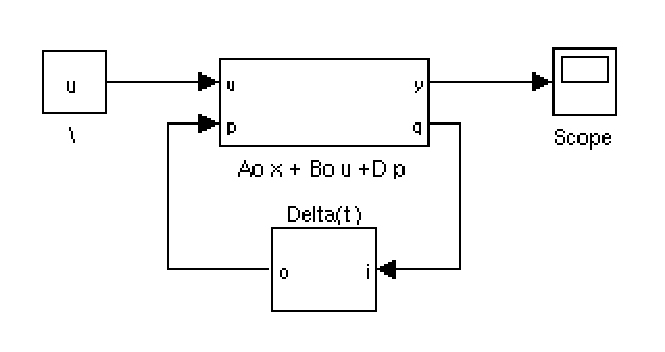
\includegraphics[width=0.60\columnwidth]{figures/carac_sis.eps}
	\caption{Sistema na forma LFT ({\it{Linear Fractional Transformation}}}
	\label{fig:carac_sist}
\end{figure}

De forma bem simplificada a matriz $A_0$ pode ser vista como a m�dia das perturba��es e
a matriz $E_A$ � a amplitude da incerteza sobre cada par�metro.

Na literatura a matriz $ \Delta(t)$ designa um bloco de incertezas {\it{n�o estruturais}}.

%===============================================================================
\subsection{Diagonais}
\label{sec:carac_diagonais}

As incertezas diagonais podem ser definidas como em (\ref{eq:carac_limit_norma_a}) e 
(\ref{eq:carac_limit_norma_b}) com a diferen�a de que o valor de $\Delta (t)$ segue
a defini��o abaixo:

\begin{equation}
\Delta (t)'\Delta (t) \leq I
\nonumber
\end{equation}

Onde:

\begin{equation}
\Delta(t)=diag(\delta_i(t)); i=1,...,ni
\nonumber
\end{equation}

A matriz $\Delta(t)$ � uma matriz quadrada de ordem $ni$.
%===============================================================================
\subsection{Elemento a elemento}
\label{sec:carac_elemento}

As incertezas de um sistema s�o elementares se  $ \mathbf{A} e \mathbf{B}$ possuem as
seguintes estruturas:

\begin{equation}
\begin{matrix}
\mathbf{A}(\Delta_e (t))\equiv A: A=A_0(s)+\Delta_A = A_0+D\Delta(t)E_A\\ 
\Delta_A(t)'\Delta_A(t) \leq I\\ \\
\mathbf{B}(\Delta_e (t))\equiv B: B=B_0(s)+\Delta_B = B_0+D\Delta(t)E_B\\  
\Delta_B(t)'\Delta_B(t) \leq I
\end{matrix}
\nonumber
\end{equation}

Onde:

\begin{equation}
\begin{matrix}
D_A=[d_{a1}\cdots d_{Anai}]; & D_B=[d_{B1}\cdots d_{Bnbi}]\\ 
E_A'=[e_{A1}' \cdots e_{Anai}' ]; & E_B'=[e_{B1}' \cdots e_{Bnbi}' ]\\ 
\Delta_A(t)=diag(\delta_{A1} \cdots \delta_{Anai}); & \Delta_B(t)=diag(\delta_{B1} \cdots \delta_{Bnbi})
\end{matrix}
\nonumber
\end{equation}

Definindo-se 

\begin{equation}
\begin{matrix}
\hat{D} \equiv [D_A \; D_B]\\ \\
\hat{E}_A \equiv \begin{bmatrix}
E_A\\ 
0_{nbi \; x\; n }
\end{bmatrix}\\ \\
\hat{E}_B \equiv \begin{bmatrix}
0_{nai \; x\; m }\\
E_B
\end{bmatrix}
\end{matrix}
\nonumber
\end{equation}

De maneira equivalente, a equa��o de estados do sistema pode ser escrito como em
(\ref{eq:carac_elem_sys}).

\begin{equation}
\begin{cases} 
\dot{x}(t)=A_0 x(t)+B_0 u(t) +\hat{D}p(t)\\ 
q(t)=\hat{E}_{a}x(t)+\hat{E}_{B}u(t)\\ 
p(t)=\Delta(t)q(t)\\ 
\Delta(t)=blocdiag(\Delta_A(t),\Delta_B(t))\\ 
p_A(t)=\Delta_A(t)q_A(t)\\ 
p_B(t)=\Delta_B(t)q_B(t)\\ 
p(t)=[p_A'(t)p_B'(t)]'\\
q(t)=[q_A'(t)q_B'(t)]' 
\end{cases}
\label{eq:carac_elem_sys}
\end{equation}

Na defini��o acima, cada bloco de incerteza $\delta_{Ai}(t)$ e $\delta_{Bj}(t)$ �
um escalar, cujo m�dulo � inferior a 1. Alem disso as matrizes $d_{Ai}$ e $d_{Bj}$
s�o vetores coluna e $e_{Ai}$ e $e_{Bj}$ s�o vetores linha.

\section{Controle Robusto}
\label{sec:robust}
%===============================================================================

Nas se��es seguintes ser� apresentado a modelagem para os tipos de incertezas.
Utilizando o sistema descrito em (\ref{eq:intro_sis}) e os limites das incertezas
descritos em (\ref{eq:intro_limit}), ser� apresentada a modelagem baseado em cada
um dos tipos apresentados a seguir.\cite{lmi_sys_control}

%===============================================================================
\subsubsection{Estabilidade quadr�tica}
\label{sec:robust_quadratic}

A ideia fundamental da estabiliza��o quadr�tica de um sistema incerto aut�nomo 
por realimenta��o linear est�tica de estados � encontrar uma lei de controle tal
que a fun��o quadr�tica definida positiva:

\begin{equation}
V(x)=x'Px; \; com P>0
\nonumber
\end{equation}

Possua sua derivada definida negativa ao longo da trajet�ria do sistema em malha fechada:

\begin{equation}
\begin{matrix}
\dot{V}(x)=x'\{(A-BK)'P+P(A-BK)\}x < 0\\ 
\forall A \in \mathbf{A}, \forall B \in \mathbf{B}
\end{matrix}
\nonumber
\end{equation}

Desta forma o que busca-se � uma matriz $P$ que satisfa�a n�o apenas uma equa��o mas
um grupo de equa��es para estabilizar o sistema de forma Robusta.

Para um sistema sem incertezas tem-se que a solu��o do problema � como abaixo:

\begin{equation}
P=W^{-1}; K=RW^{-1}
\nonumber
\end{equation}

Para o sistema abaixo com $R\equiv KP^{-1}$.

\begin{equation}
WA_0'+A_0W -B_0R-R'B_0 < 0
\nonumber
\end{equation}

%===============================================================================
\subsection{Polit�pica}
\label{sec:robust_politopica}

Para o caso de incertezas do tipo polit�pico uma condi��o necess�ria e suficiente para a
estabilidade quadr�tica do sistema incerto aut�nomo em malha fechada � que todos os v�rtices
do poliedro que constituem o conjunto de modelos possuam a mesma matriz $P$ sim�trica
definida positiva como matriz de Lyapunov.

\begin{equation}
WA_i'+A_iW-B_jR-R'B_j'< 0
\label{eq:robust_politopico}
\end{equation}

Para $\forall i=1,...,na, \forall j=1,...,nb$.

O sistema utilizado neste trabalho (\ref{eq:intro_sis}) � caracterizado utilizando a
forma polit�pica como em (\ref{eq:carac_sis_politopico}).

\begin{equation}
\begin{matrix}
A_1=\begin{bmatrix}
0 & 1\\ 
-ba_1 &a_1+b 
\end{bmatrix} \; A_2=\begin{bmatrix}
0 & 1 \\ 
-ba_2 & a_2+b 
\end{bmatrix}
\\ \; & \; \\
B_1=\begin{bmatrix}
0\\ 
k_1
\end{bmatrix}B_2=\begin{bmatrix}
0\\ 
k_2
\end{bmatrix}
\end{matrix}
\label{eq:carac_sis_politopico}
\end{equation}

A partir de (\ref{eq:robust_politopico}) tem-se o conjunto de inequa��es lineares apresentado
em (\ref{eq:robust_politopico_equations}).

\begin{equation}
\begin{matrix}
WA_1'+A_1W-B_1R-R'B_1'<0\\ 
WA_1'+A_1W-B_2R-R'B_2'<0\\ 
WA_2'+A_2W-B_1R-R'B_1'<0\\ 
WA_2'+A_2W-B_2R-R'B_2'<0
\end{matrix}
\label{eq:robust_politopico_equations}
\end{equation}

%===============================================================================
\subsection{Limitada em norma}
\label{sec:carac_limit_norma}

Considerando o sistema apresentado em (\ref{eq:robust_sis_incert}) com $\omega(t) \equiv 0$.

\begin{equation}
\begin{cases}
\dot{x}(t)=A_0x(t)+B_0u(t)B_{\omega}\omega(t)+Dp(t)
\\ 
q(t)=E_Ax(t)+E_Bu(t)+Fp(t)
\\ 
z(t)=Gx(t)+Hu(t)
\\
p(t)=\Delta(t)q(t); \; \left \| \Delta(t) \right \| \leq 1
\end{cases}
\label{eq:robust_sis_incert}
\end{equation}

Para este sistema temos que a derivada da fun��o $V(x)=x'Px$ seja definida positiva:

\begin{equation}
x'-(A_0-B_0 K)'P-P(A_0-B_0 K)x-x'PDp-p'D'Px < 0
\nonumber
\end{equation}

Para todo $x \neq 0$ tal que $p'p \leq q'q$ implica de maneira equivalente:

\begin{equation}
p'p \leq ((E_A-E_B K)x)'(E_A-E_B K)x
\nonumber
\end{equation}

Tem-se ent�o que o sistema apresentado em (\ref{eq:robust_limit_norma}) � uma condi��o
necess�ria e suficiente para a estabilidade quadr�tica do sistema com incertezas limitadas
em norma e tamb�m � convexa, portanto pode ser resolvida com algoritmos de resolu��o de LMI.

\begin{equation}
\begin{bmatrix}
-A_0+B_0R-WA_0'+R'B_0'-DD' & -(WE_A+RE_B')\\ 
-(WE_A'+R'E_B')' & I
\end{bmatrix}>0
\label{eq:robust_limit_norma}
\end{equation}

Desta forma para o sistema (\ref{eq:intro_sis}) temos que a modelagem para incertezas limitadas
em norma � a apresentada em (\ref{eq:robust_sis_limit}).

\begin{equation}
\begin{matrix}
A_0=\begin{bmatrix}
0 & 1\\ 
-b(a_1+a_2)/2 & b+(a_1+a_2)/2
\end{bmatrix} 
\\
\;
\\
B_0=\begin{bmatrix}
0\\ 
(k_1+k_2)/2
\end{bmatrix}
\\
\; 
\\
E_A=\begin{bmatrix}
(a_1-a_2)/2 & 0\\ 
0 & (a_1-a_2)/2
\end{bmatrix} 
\\
\;
\\
D=\begin{bmatrix}
0 & 0\\ 
1 & 1
\end{bmatrix}
\\
\;
\\
E_B=\begin{bmatrix}
0\\ 
(k_1-k_2)/2
\end{bmatrix}
\end{matrix}
\label{eq:robust_sis_limit}
\end{equation}


%===============================================================================
\subsection{Diagonais}
\label{sec:carac_diagonais}

Para incertezas diagonais o sistema fica como em (\ref{eq:robust_sis_limit}).

%===============================================================================
\subsection{Elemento a elemento}
\label{sec:carac_elemento}

Para as incertezas do tipo elemento a elemento temos as seguintes defini��es:

\begin{equation}
\begin{matrix}
D_A=\begin{bmatrix}
0\\ 
1
\end{bmatrix}
\\ 
E_A=\begin{bmatrix}
(a_1-a_2)/2 & (a_1-a_2)/2
\end{bmatrix}
\\ \\
D_B=\begin{bmatrix}
0\\ 
1
\end{bmatrix}\\
E_B=[(k_1-k_2)/2]
\end{matrix}
\nonumber
\end{equation}

Desta forma chega-se:

\begin{equation}
\begin{matrix}
\hat{D} = \begin{bmatrix}
0 & 0\\ 
1 & 1
\end{bmatrix}\\ \\
\hat{E}_A = \begin{bmatrix}
(a_1-a_2)/2 & (a_1-a_2)/2\\ 
0 & 0
\end{bmatrix}\\ \\
\hat{E}_B =\begin{bmatrix}
0\\ 
(k_1-K2)/2
\end{bmatrix}\\ \\
\Delta(t)=\begin{bmatrix}
\delta_A(t) &0 \\ 
0 & \delta_B(t)
\end{bmatrix}
\end{matrix}
\nonumber
\end{equation}


%===============================================================================
\section{Minimiza��o da norma $H_2$}
\label{sec:normH2}

Considerando o sistema apresentado em (\ref{eq:robust_sis_incert}) em malha fechada
com $\Delta \equiv 0$ e condi��o inicial nula. Um crit�rio normalmente utilizado 
� a norma $H_2$ da fun��o de transfer�ncia entre a entrada das perturba��es $\omega$
e a sa�da $z$. A norma $H_2$ pode ser calculada como em (\ref{eq:normh2_def}).

\begin{equation}
\left \| T(s) \right \|_2 \equiv \gamma _2=\sqrt{Tr(B_{\omega}'P_o B_{\omega})}
\label{eq:normh2_def}
\end{equation}

Onde :

\begin{equation}
P_o=\int_{0}^{\infty}((G-HK))e^{(A_0-BK)}B_{\omega})'((G-HK))e^{(A_0-BK)}B_{\omega})dt
\nonumber
\end{equation}

{\it{Interpreta��o estoc�stica da norma $H_2$}}: Se considerarmos $\omega(t)$ como sendo 
ruido branco, ent�o a norma $H_2$ de $T(s)$ � o valor da vari�ncia assint�tica da sa�da $z(t)$:

\begin{equation}
\left \| T(s) \right \|_2=\sqrt{\lim_{t\rightarrow \infty}E(z(t)'z(t))}
\nonumber
\end{equation}

{\it{Interpreta��o determin�stica da norma $H_2$}}: D� a ideia da energia da sa�da $z(t)$ 
em resposta as condi��es iniciais nulas.

\begin{equation}
\int_{0}^{\infty}z(t)'z(t)dt=x_0'P_o x_0
\nonumber
\end{equation}

Assim tendo que a norma pode ser apresentada como a seguir:

\begin{equation}
\left \| T(s) \right \|_2=\sqrt{\sum_{i=1}^{n_w} \int_{0}^{\infty}\left \| z^{i}(t) \right \|^2 dt}
\nonumber
\end{equation}

%===============================================================================
\subsection{$H_2$ - Sistemas Lineares sem incertezas}
\label{sec:h2_sis_lin_sem_incertezas}

Se considerarmos o sistema (\ref{eq:robust_sis_incert}) com condi��es iniciais nulas e $\Delta \equiv 0$
temos o sistema apresentado em (\ref{eq:normh2_sis_sem_incertezas}).

\begin{equation}
\begin{cases}
\dot{x}(t)=(A_0-B_0 K)x(t)+B_{\omega}\omega(t)
\\
z(t)=(G-HK)x(t)
\end{cases}
\label{eq:normh2_sis_sem_incertezas}
\end{equation}

Pode-se desta forma minimizar o escalar $\gamma_2$ sujeito a (\ref{eq:normh2_relim}).

\begin{equation}
\begin{matrix}
\gamma_2^2 > Tr(M)
\\ 
\\
\begin{bmatrix}
M & B_{\omega}'\\ 
B_{\omega} & W
\end{bmatrix} > 0
\\ 
\\ 
\begin{bmatrix}
-WA_0'+R'B_0'-A_0W +B_0R & (GW-HR)' \\ 
(GW-HR) & I
\end{bmatrix} >0
\end{matrix}
\label{eq:normh2_relim}
\end{equation}

%===============================================================================
\subsection{$H_2$ - Incertezas do tipo polit�pico}
\label{sec:normh2_politopico}

Para um sistema com incertezas do tipo politopico ter garantia do limite superior de $\gamma_2$ 
para a norma $H_2$ de todos os sistemas pertencentes ao conjunto de sistemas formados pelas
incertezas � satisfeita para:

\begin{equation}
\begin{matrix}
\gamma_2^2 > Tr(M)
\\ 
\\
\begin{bmatrix}
M & B_{\omega}'\\ 
B_{\omega} & W
\end{bmatrix} > 0
\\ 
\\ 
\begin{bmatrix}
-WA_i'+R'B_j'-A_i W +B_j R & (GW-HR)' \\ 
(GW-HR) & I
\end{bmatrix} >0
\\
\forall i=1,...,na
\\
\forall j=1,...,nb
\end{matrix}
\label{eq:normh2_polytopic}
\end{equation}
%===============================================================================
\subsubsection{Simula��o}

A resolu��o do sistema de LMIs (\ref{eq:normh2_polytopic}) gerou os seguintes resultados:

\begin{equation}
\begin{matrix}
W=\begin{bmatrix}
5.3185 &  -1.0406\\
-1.0406 & 938.1095
\end{bmatrix}\\ \\ 
R=1.10^6\begin{bmatrix}
0.0008 &  -1.3383
\end{bmatrix}
\\ \\
K=1.10^3\begin{bmatrix}
-0.1259 &  -1.4267
\end{bmatrix}
\\ \\
M =  2.3045e-12
\end{matrix}
\nonumber
\end{equation}

A simula��o do sistema em malha fechada com o ganho $K$ encontrado obtem a resposta
apresentada na Figura (\ref{fig:h2_polytopic}), O sistema simulado com as incertezas
sendo utilizadas com o valor mediano � apresentada na linha $A0_B0$, para os sistemas
que possuem as 4 combina��es de matrizes $A_1, A_2, B_1, B_2$ que formam os v�rtices
do politopo, s�o apresentados nas demais linhas do gr�fico.

\begin{figure}[htbp]
	\center
	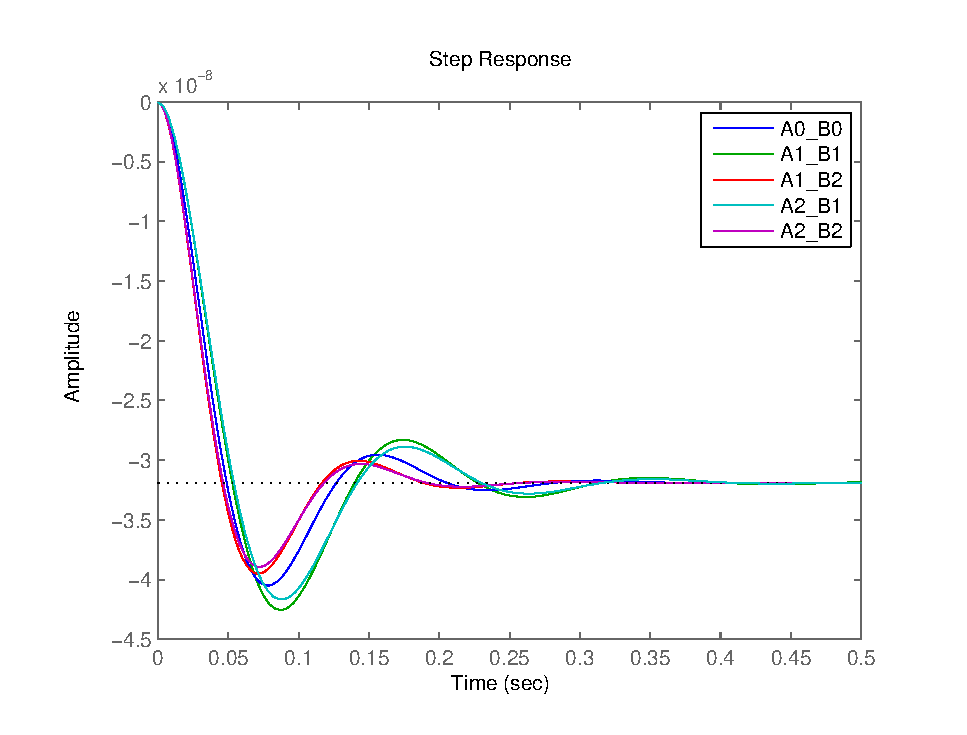
\includegraphics[width=1\columnwidth]{figures/h2_polytopic.eps}
	\caption{Resposta do sistema (\ref{eq:sis_mf_incerteza}) com o ganho K encontrado 
		pelo crit�rio de $H_2$, para incertezas do tipo politopicas.}
	\label{fig:h2_polytopic}
\end{figure}

%===============================================================================
\subsection{$H_2$ - Incertezas limitadas em norma}
\label{sec:normh2_norm_limit}

Para o caso de incertezas com norma limitada temos (\ref{eq:normh2_norm_limit}).


\begin{equation}
\begin{matrix}
\gamma _2^2 > Tr(B_{\omega}'W^{-1}B_{\omega})
\\ 
\\
\begin{bmatrix}
Y & (E_AW-E_BR)' & (GW-HR)'\\ 
(E_AW-E_BR) & I & 0\\ 
 (GW-HR) & 0 & I
\end{bmatrix} \geq 0
\\ 
\\ 
Y=-WA_0'+R'B_0'-A_0W +B_0R -DD'
\end{matrix}
\label{eq:normh2_norm_limit}
\end{equation}

Com a realimenta��o $K=RW^{-1}$.
%===============================================================================
\subsubsection{Simula��o}

A resolu��o do sistema de LMIs (\ref{eq:normh2_norm_limit}) gerou os seguintes resultados:

\begin{equation}
\begin{matrix}
W=\begin{bmatrix}
0.4644 &  -0.0305\\
-0.0305 &   0.7975
\end{bmatrix}\\ \\ 
R=1.10^3\begin{bmatrix}
0.0009 &  -8.6987
\end{bmatrix}
\\ \\
K=1.10^4\begin{bmatrix}
-0.0716 &  -1.0935
\end{bmatrix}
\\ \\
M =  0.0170
\\
\lambda_1=-0.0326\\
\lambda_2=-1.7666
\end{matrix}
\nonumber
\end{equation}

A simula��o do sistema em malha fechada com o ganho $K$ encontrado obtem a resposta
apresentada na Figura (\ref{fig:h2_norm_bounded}). Os valores de $\lambda_1$ e $\lambda_2$ 
s�o os autovalores do sistema em malha fechada ($A0_B0$). As demais linhas apresentadas no
gr�fico s�o relativas ao sistema em v�rtices das incertezas, afim de compara��o com o sistema
no centro das incertezas.

\begin{figure}[htbp]
	\center
	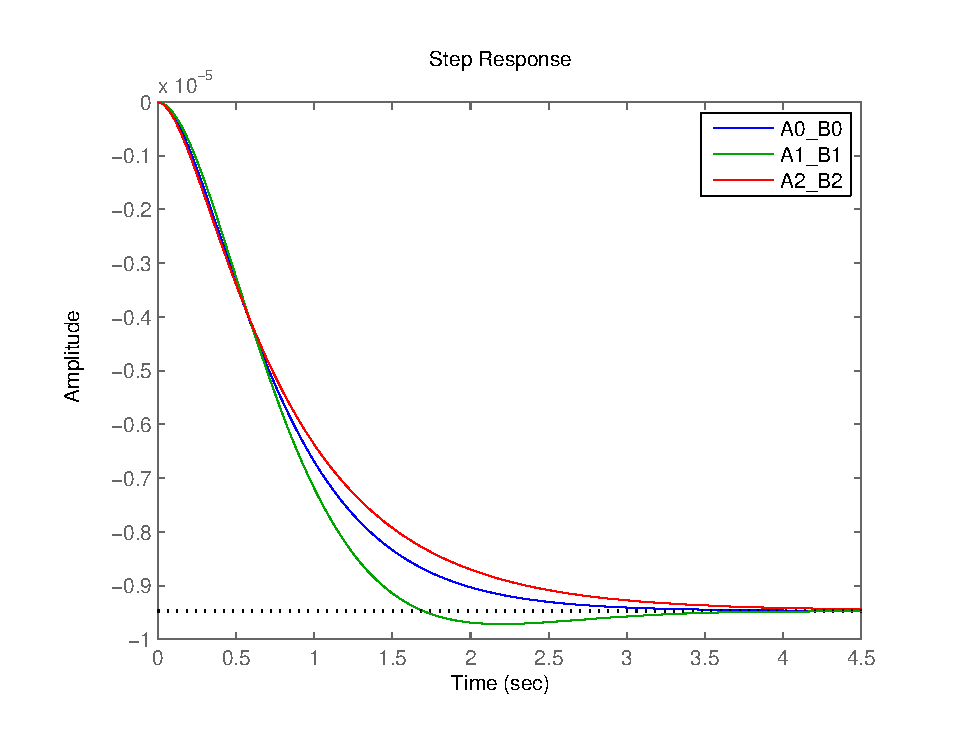
\includegraphics[width=1\columnwidth]{figures/h2_norm_bounded.eps}
	\caption{Resposta do sistema (\ref{eq:sis_mf_incerteza}) com o ganho K encontrado 
		pelo crit�rio de $H_2$ para incertezas do tipo limitadas em norma.}
	\label{fig:h2_norm_bounded}
\end{figure}

%===============================================================================
\section{Norma $H_{\infty}$}
\label{sec:normHinf}

Para o sistema apresentado em (\ref{eq:robust_sis_incert}) a norma $L_2$ deste sistema
� definido como em (\ref{eq:normhinf_l2}).

\begin{equation}
\underset{\left \| \omega(t) \right \|_2 \neq 0}{sup}=\frac{\left \| z(t) \right \|_2}{\left \| \omega(t) \right \|_2}
\label{eq:normhinf_l2}
\end{equation}

Onde a norma $L_2$ de um sinal $\omega(t)$ � definida como abaixo:

\begin{equation}
\left \| \omega(t) \right \|_2 \equiv \sqrt{\int_{0}^{\infty}\omega(t)'w(t) dt}
\nonumber
\end{equation}

Suponha que exista uma fun��o quadr�tica positiva $V(x)=x'Px$ com $P=P'>0$ e um escalar positivo
$\gamma_{\infty}$ tal que:


\begin{equation}
\dot{V}z(t)'z(t)-\gamma_{\infty}^{\omega}\omega(t)'\omega(t)\leq 0
\nonumber
\end{equation}
%===============================================================================
\subsection{$H_{\infty}$ - Sistemas Lineares sem incertezas}
\label{sec:hinf_sis_lin_sem_incertezas}

Considerando o sistema apresentado em (\ref{eq:robust_sis_incert}) em malha fechada, com 
condi��o inicial nula ($x(0)\equiv 0$) e com $ \Delta (t) \equiv 0$, obt�m-se desta forma
o sistema apresentado em (\ref{eq:sis_mf_incerteza}).

\begin{equation}
\begin{cases}
\dot{x}(t)=(A_0-B_0K)x(t)+B_{\omega}\omega(t)\\ 
z(t)=(G-HK)x(t)
\end{cases}
\label{eq:sis_mf_incerteza}
\end{equation}

A LMI que deve ser satisfeita para que a condi��o de $H_{\infty}$ seja obtida � apresentada
em (\ref{eq:hinf_sem_incerteza}).

\begin{equation}
\begin{matrix}
\begin{bmatrix}
Y & -(GW-HR)'\\ 
 -(GW-HR) & \gamma_{\infty}^2 I  
\end{bmatrix}\geq 0
\\ \\
Y= -WA_0'+R'B_0'-A_0W-B_0R-B_{\omega}B_{\omega}'
\end{matrix}
\label{eq:hinf_sem_incerteza}
\end{equation}

Assim pode-se garantir o limite superior minimo para o ganho $L_2$ do sistema 
(\ref{eq:sis_mf_incerteza}).

Para o caso de sistemas lineares invariantes no tempo a otimiza��o d� exatamente o valor do
ganho $L_2$ que � igual a norma $H_{\infty}$. 

\begin{equation}
T(s)=(G-HK)(sI-(A_0-B_0K))^{-1}B_{\omega}
\nonumber
\end{equation}

Que � equivalente a:

\begin{equation}
\left \| T(s) \right \|_{\infty} \equiv \underset{\omega \in \Re}{max}\sqrt{\lambda (T'(j\omega)T(j\omega))}
\nonumber
\end{equation}

%===============================================================================
\subsection{$H_{\infty}$ - Incertezas do tipo polit�pico}
\label{sec:hinf_sis_politopico}

No caso de incertezas do tipo polit�picas o limite superior minimo para o ganho $L_2$ pode ser
definido pela equa��o (\ref{eq:hinf_sis_politopico}).

\begin{equation}
\begin{matrix}
\begin{bmatrix}
Y & -(GW-HR)'\\ 
-(GW-HR) & \gamma_{\infty}^2
\end{bmatrix}\geq 0
\\ 
\\ 
Y=-WA_i'+R'B_j'-A_iW+B_jR-B_{\omega}B_{\omega}'
\\ \\
W>0
\end{matrix}
\label{eq:hinf_sis_politopico}
\end{equation}

%===============================================================================
\subsubsection{Simula��o}

A resolu��o do sistema de LMIs (\ref{eq:hinf_sis_politopico}) gerou os seguintes resultados:

\begin{equation}
\begin{matrix}
W=\begin{bmatrix}
0.0012 &  -0.6805\\
-0.6805 & 390.6637
\end{bmatrix}\\ \\ 
R=1.10^8\begin{bmatrix}
-0.0458 &  -9.9849
\end{bmatrix}
\\ \\
K=1.10^12\begin{bmatrix}
-2.4902 &  -0.0043
\end{bmatrix}
\\ \\
\gamma_{\infty}^2 =2.1730e-11
\end{matrix}
\nonumber
\end{equation}

A simula��o do sistema em malha fechada com o ganho $K$ encontrado obtem a resposta
apresentada na Figura (\ref{fig:h2_polytopic}). O sistema simulado com as incertezas
sendo utilizadas com o valor mediano � apresentada na linha $A0_B0$, para os sistemas
que possuem as 4 combina��es de matrizes $A_1, A_2, B_1, B_2$ que formam os v�rtices
do politopo, s�o apresentados nas demais linhas do gr�fico.

\begin{figure}[htbp]
	\center
	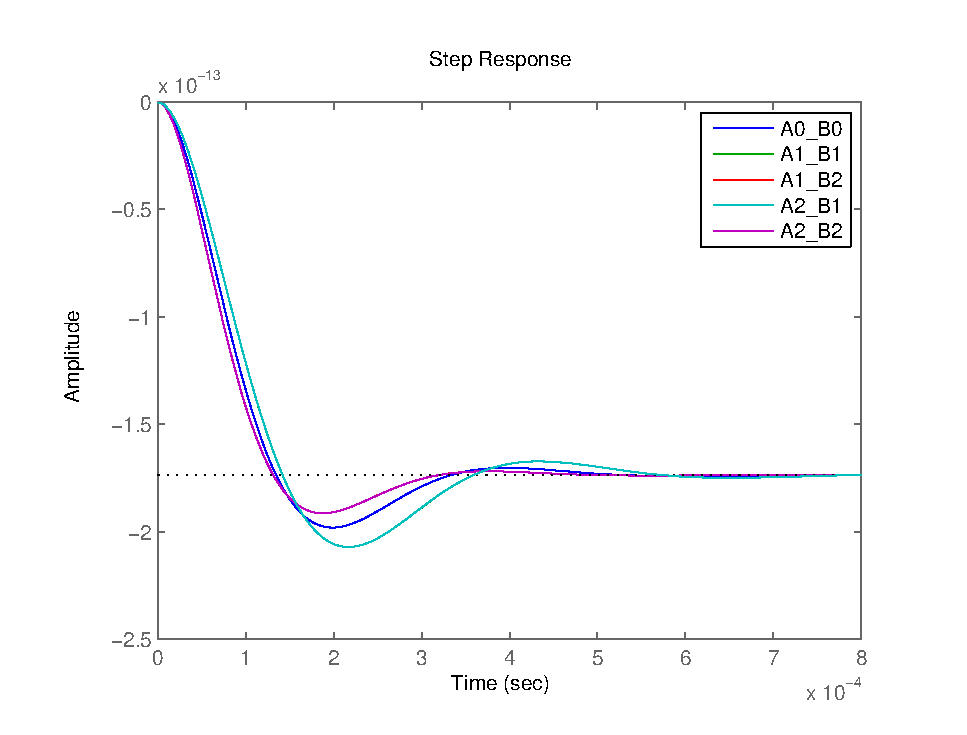
\includegraphics[width=0.95\columnwidth]{figures/hinf_polytopic.eps}
	\caption{Resposta do sistema (\ref{eq:sis_mf_incerteza}) com o ganho K encontrado 
		pelo crit�rio de $H_{\infty}$, para incertezas do tipo Politopicas.}
	\label{fig:hinf_polytopic}
\end{figure}


%===============================================================================
\subsection{$H_{\infty}$ - Incertezas limitadas em norma}
\label{sec:hinf_sis_norm_limit}

Considerando o sistema descrito em (\ref{eq:robust_sis_incert}) com $\left \| \Delta(t) \right \|\leq 1$.
A condi��o descrita em (\ref{eq:hinf_sem_incerteza}) � equivalente a (\ref{eq:hinf_sis_norm_lim}).

\begin{equation}
\begin{matrix}
\begin{bmatrix}
Y &(E_AW-E_BR)' & -(GW-HR)'\\ 
(E_AW-E_BR) & I & 0\\
-(GW-HR) & 0& \gamma_{\infty}^2
\end{bmatrix}\geq 0
\\ 
\\ 
Y=-WA_0'+R'B_0'-A_0W+B_0R-B_{\omega}B_{\omega}'
\\ \\
W>0
\end{matrix}
\label{eq:hinf_sis_norm_lim}
\end{equation}

Satisfazendo a equa��o (\ref{eq:hinf_sis_norm_lim}) obt�m-se o limite superior minimo para o
ganho $L_2$ e se o sistema for linear e invariante no tempo este valor ser� o mesmo da norma 
$H_{\infty}$ da fun��o de transfer�ncia entre $\omega$ e $z$.

%===============================================================================
\subsubsection{Simula��o}

A resolu��o do sistema de LMIs (\ref{eq:hinf_sis_norm_lim}) gerou os seguintes resultados:

\begin{equation}
\begin{matrix}
W=\begin{bmatrix}
0.2449 & -0.0315\\
-0.0315 &   0.8360
\end{bmatrix}\\ \\ 
R=1.10^3\begin{bmatrix}
 0.0010 & -7.8417
\end{bmatrix}
\\ \\
K=1.10^3\begin{bmatrix}
-1.2096 &  -9.4257
\end{bmatrix}
\\ \\
\gamma_{\infty}^2 = 0.07
\\
\lambda_1=-0.0529\\
\lambda_2=-1.6550
\end{matrix}
\nonumber
\end{equation}

A simula��o do sistema em malha fechada com o ganho $K$ encontrado obtem a resposta
apresentada na Figura (\ref{fig:hinf_norm_bounded}). Os valores de $\lambda_1$ e $\lambda_2$ 
s�o os autovalores do sistema em malha fechada ($A0_B0$). As demais linhas apresentadas no
gr�fico s�o relativas ao sistema em v�rtices das incertezas, afim de compara��o com o sistema
no centro das incertezas.

\begin{figure}[htbp]
	\center
	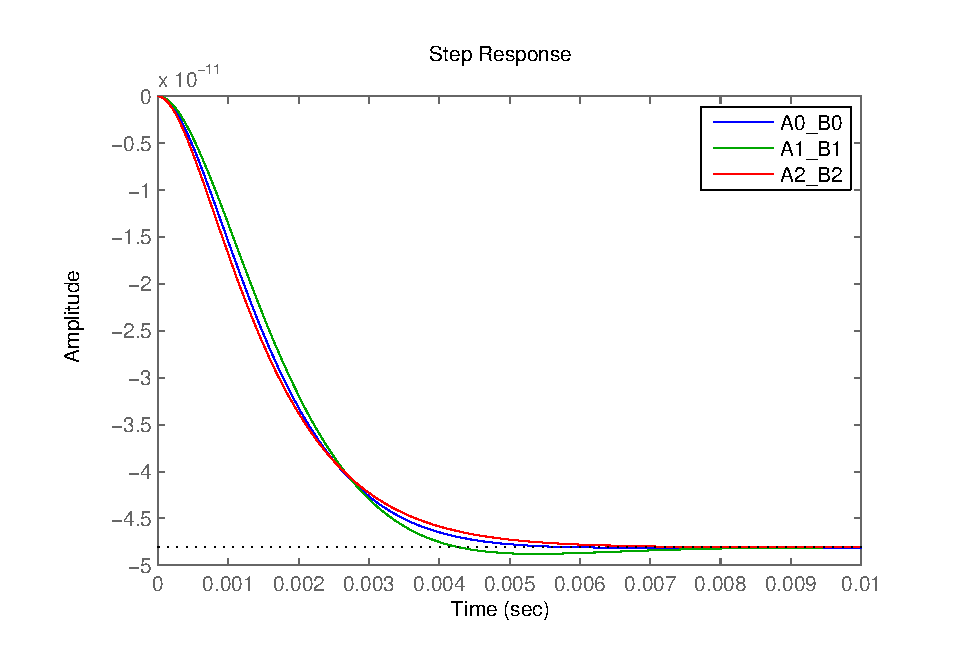
\includegraphics[width=0.95\columnwidth]{figures/hinf_norm_bounded.eps}
	\caption{Resposta do sistema (\ref{eq:sis_mf_incerteza}) com o ganho K encontrado 
		pelo crit�rio de $H_{\infty}$, para incertezas do tipo limitadas em norma.}
	\label{fig:hinf_norm_bounded}
\end{figure}


%===============================================================================

\section{Conclus�es}
\label{sec:concl}

O projeto de controladores denominados Robustos � uma �rea bem abrangente e com
in�meras aplica��es na engenharia de controle. Sistemas sujeitos a incertezas s�o
praticamente todos os sistemas f�sicos, alguns com mais e outros com menos intensidade
e representatividade da incerteza apresentada. Estas incertezas como vimos pode ser
de v�rias origens (Se��o \ref{sec:caracterization}) e s�o classificadas em tipos. Neste
trabalho apresentamos a modelagem matem�tica de 4 tipos, considerados principais e
que cobrem boa parte das incertezas mais encontradas.

Incertezas do tipo polit�picas (Se��o \ref{sec:carac_politopica}) formam uma regi�o em forma de 
um politopo, e para se encontrar uma realimenta��o de estados para este sistema � 
necess�rio que o sistema seja est�vel em todos os v�rtices deste politopo. Nas se��es 
\ref{sec:normh2_politopico} e \ref{sec:hinf_sis_politopico} foi apresentado uma
realimenta��o de estados para incertezas deste tipo tendo como requisitos as normas 
$H_2$ e $H_{\infty}$ respectivamente. Foi observado pelas Figuras (\ref{fig:h2_polytopic})
e (\ref{fig:hinf_polytopic}) que o sistema que � submetido a norma $H_2$ possui um
sobrepasso maior para uma entrada do tipo degrau, e um tempo de acomoda��o maior
se comparado com o sistema sujeito a norma $H_{\infty}$.

Incertezas do tipo limitadas em norma (Se��o \ref{sec:carac_limit_norma}) onde n�o se tem 
informa��es detalhadas sobre os componentes do sistema. Para este tipo de incerteza se 
encontrou uma realimenta��o de estados sujeito as normas $H_2$ e $H_{\infty}$ e 
nas Figuras (\ref{fig:h2_norm_bounded}) e (\ref{fig:hinf_norm_bounded}) observa-se o
comportamento do sistema nos dois casos, com o sistema no centro das incertezas e tamb�m 
em algum dos v�rtices das incertezas.

Apresentou-se tamb�m a modelagem matem�tica para incertezas do tipo Diagonais 
(Se��o \ref{sec:carac_diagonais}) e elemento a elemento (Se��o \ref{sec:carac_elemento}).

Sa Se��o \ref{sec:robust} foi apresentado resumidamente a modelagem matem�tica utilizada
para resolver o problema de estabilidade dos sistemas sujeitos a cada uma das incertezas
retratadas neste trabalho.

Para a resolu��o dos problemas de incertezas para cumprimento das normas especificadas
foi utilizado o Solver de LMI \cite{lmi_matlab} do Matlab. A ferramenta � muito interessante e facilita 
muito o projeto e resolu��o da problem�tica que envolve sistemas mais complexos e com
mais incertezas em sua formula��o.

Controladores robustos s�o muitas vezes n�o s� desejados, mas tamb�m necess�rios em certos
tipos de aplica��es. Desta forma o estudo de modelagem, caracteriza��o e resolu��o destes
problemas se torna muito importante. O conhecimento matem�tico dos m�todos que as ferramentas
atuais utilizam para resolu��o dos problemas � tamb�m muito importante e �til para 
qualquer engenheiro que venha a se deparar com problemas incertos e com requisitos de
confiabilidade elevados.




\bibliographystyle{IEEEtran}
\bibliography{biblio}

\end{document}
